\chapter{How Are You Going to Make Money? The Business/Venture Model}

This lecture, given by Rich Kivel in Joseph Hadzima's MIT OpenCourseWare course and curated here by LazyingArt LLC, begins exactly where customer discovery leaves off. Bob Jones had already shown that different customers and different prices begin to define a business. Kivel now asks the harder operational question: once we have an invention, a service, or a piece of technology, how does it become revenue, investor return, and finally a sustainable business? The lecture answers this in a deliberate order. We are first shown an operating story, then given a definition, then led through large platform cases, and finally brought back to industry-specific pressure, where the problem of adoption becomes sharper than the problem of invention.

\section{From Customer Discovery to Business Model}

Kivel opens by refusing to treat the business model as branding language or venture-capital mythology. It is the practical continuation of customer discovery. If the previous lecture asked who the customer is and what price they may tolerate, this lecture asks how an offering reaches the point at which money actually returns to the company.

A compact way to state the lecture's practical target is
\begin{equation}
\text{technology} \to \text{distribution} \to \text{adoption} \to \text{revenue} \to \text{sustainable business}.
\end{equation}
This equation is not spoken symbolically in the room, but it captures the direction of the lecture. The first term by itself is never enough. An invention sitting in a lab is not yet a business. Between invention and sustainability there lie channels, users, pricing, behavior, and scale.

Kivel's own setup matters. He introduces himself not as a theorist of models but as an operating executive who moved through sales, marketing, partnerships, CEO work, and later investing. That operating emphasis is the governing tone of the lecture. We are to think about business models not from the top down but from the point at which the product must meet a buyer.

\section{MolecularWare and the First Operating Model}

The first real lesson comes through the MolecularWare story. The company emerged in the era of the Human Genome Project. Labs were filled with scanners, robots, refrigerators, and other instruments, each with its own computer and its own software. The technical problem looked, at first glance, like a software problem. But Kivel is careful: the commercial problem is wider. If the instruments cannot speak to each other, then the scientists are forced into spreadsheets, manual import and export, and eventually chaos.

The lecture breaks the product logic into a clean sequence:
\begin{equation}
\text{capture} \to \text{visualize} \to \text{data mine} \to \text{create value}.
\end{equation}
This is one of the most useful compact constructions in the lecture. The company first captures the data coming off the instruments. It then makes the data visible and interpretable. Only after that can one mine the data and extract value. Kivel's point is that the value does not reside merely in the machine, nor even in the raw information. It resides in making the information usable.

\begin{figure}[htbp]
\centering
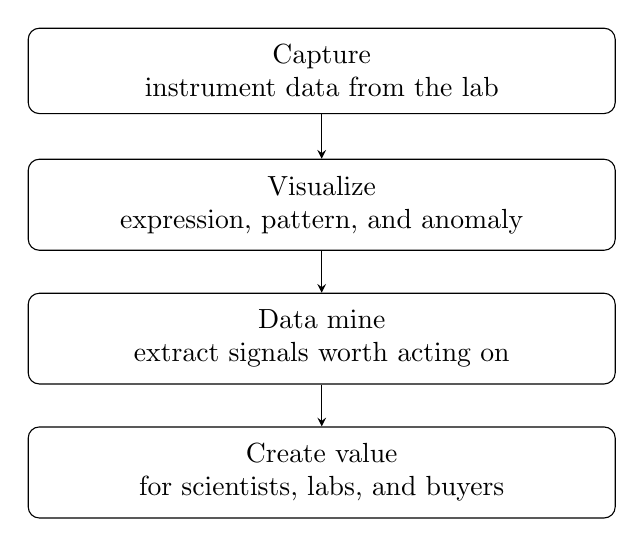
\begin{tikzpicture}[>=stealth]
\node[draw, rounded corners, align=center, text width=0.58\linewidth, inner sep=6pt] (a) at (0,0) {Capture\\instrument data from the lab};
\node[draw, rounded corners, align=center, text width=0.58\linewidth, inner sep=6pt] (b) at (0,-1.7) {Visualize\\expression, pattern, and anomaly};
\node[draw, rounded corners, align=center, text width=0.58\linewidth, inner sep=6pt] (c) at (0,-3.4) {Data mine\\extract signals worth acting on};
\node[draw, rounded corners, align=center, text width=0.58\linewidth, inner sep=6pt] (d) at (0,-5.1) {Create value\\for scientists, labs, and buyers};
\draw[->] (a) -- (b);
\draw[->] (b) -- (c);
\draw[->] (c) -- (d);
\end{tikzpicture}
\caption{Transcript-derived reconstruction of the MolecularWare value chain.}
\end{figure}

That is the product side. The lecture then moves, without breaking stride, to the channel side. MolecularWare originally sold to academics, because those were the people the founders knew. This is a perfectly natural starting point and a poor scaling model. A company whose entire client base is one narrow class of buyer is difficult to scale and difficult to finance. So the channel itself had to evolve:
\begin{equation}
\text{direct to academics} \to \text{distributors} \to \text{OEM}.
\end{equation}

The first extension was through Asian distributors, because building a direct sales force in Asia was out of the question for a Kendall Square company with roughly fifteen people. Distributors therefore did not merely accelerate sales; they changed the business model by making a new geography reachable.

The second extension was OEM. Here the logic becomes even cleaner. MolecularWare had strong software and weak incentives to build instruments. Other companies had good instruments and poor software. Bundle the software into the instrument, let the instrument manufacturer do the expensive selling, and collect revenue whenever the instrument moves.

\subsection{Question \& Answer}

\paragraph{Question.} What is OEM, and why did it materially change the company?

\paragraph{Answer.} OEM means original equipment manufacturer. In the lecture, this is not just a definition but a structural shift. MolecularWare stops trying to sell every installation itself. Instead, it places its software inside another firm's instrument. The instrument company carries the burden of manufacturing, channel access, and much of the selling process. MolecularWare receives value each time the bundled instrument is sold. The route to market changes, and with it the economics of growth.

One sees already the central rhythm of the lecture: invention, yes, but invention coupled to the question of who already reaches the buyer, who controls the channel, and who can convert technical quality into repeated payment.

\section{Definition, Flexibility, and the Nine-Part Canvas}

Only after the operating story does Kivel stop to give the definition. This ordering is important. We are not handed a static framework and then asked to illustrate it. We are shown a company in motion, and only then is the abstraction supplied.

\begin{definition}
A business model describes the rationale by which an organization creates, delivers, and captures value.
\end{definition}

A faithful symbolic compression of the spoken definition is
\begin{equation}
\text{Business model}=\text{create value}+\text{deliver value}+\text{capture value}.
\end{equation}

\begin{remark}
The lecture states this in words, not as a displayed equation. The symbolic form is useful because it keeps the three pieces coupled. One does not create value and then hope that delivery and capture will somehow take care of themselves.
\end{remark}

Kivel then leans on the \emph{Business Model Generation} canvas and immediately warns against a common mistake. The nine components are not equal-sized permanent boxes. Their weight changes with product development, financing, timing, and company stage. One can hear the operating executive in the way he phrases it: these components ``blend together,'' and they must move harmoniously.

His growth sequence is stated in headcount rather than in abstract scaling language:
\begin{equation}
8 \to 85 \to 250 \to 1{,}000 \ \text{people}.
\end{equation}
He attributes this kind of growth not merely to being well funded, but to having a model flexible enough to absorb new scale. That is the real point of the canvas in this lecture. It is not a filing system. It is a coupled machine.

The orchestra metaphor makes the same point from another angle. If the value proposition, customer segments, cost structure, activities, and resources move together, the system works. If one part falls behind, second- and third-order consequences appear. In Kivel's language, once the cost structure drifts out of alignment, support degrades, repeat business weakens, and the model starts to damage itself.

\section{A Menu of Canonical Models}

With the operating case and the formal definition in hand, the lecture broadens. Kivel now says, in effect, that none of this should feel alien. We all live among business models every day.

The main families named in the lecture are the following:
\begin{itemize}
\item subscription,
\item freemium,
\item marketplace,
\item advertising,
\item direct sales,
\item reseller,
\item OEM.
\end{itemize}

The important teaching move here is not classification for its own sake. Kivel is re-educating perception. A business model is not exotic terminology. It is the ordinary structure by which a firm reaches the market and gets paid.

The subscription example is introduced through a contrast with the old Blockbuster world. One once drove to the store, rented a tape or disc, returned it, and ended the transaction. Subscription logic emerges only when the economy shifts from owning particular units to maintaining access to an experience. The freemium model extends the same idea in another direction: give initial access away, then charge later, often in a recurring way. The marketplace model lets many small sellers participate through a larger platform. Advertising transforms attention into revenue rather than requiring equal direct payment from every user.

The older structures remain alive as well. Direct sales, reseller arrangements, and OEM are not relics. Indeed, Kivel stresses that in fields such as pharmaceutical biotech, direct selling survives because doctors are busy, conferences are limited, and the firm must physically educate the buyer. The Intel example sharpens this further: Intel does not care about retail intimacy with end users. It sells to manufacturers. In the lecture's improvised language, it is not merely business-to-business but almost business-to-manufacturer.

Thus by the time we leave this section, the audience has been taught to see what was already in front of them.

\section{Netflix and the Logic of Model Revision}

Netflix is the lecture's central example of survival by modification. The story begins with Blockbuster, whose stores once dominated the world of video rental. Netflix enters not as a movie studio, not as a global streaming empire, but as a company that mails DVDs. This seems almost modest until one sees the business logic. Physical retail stores are expensive. Warehouses plus mailing are cheaper. Late fees disappear. Inventory is centralized. Convenience rises.

Bandwidth constraints explain why the first model was mail rather than streaming. Kivel is explicit: at the beginning, downloading a feature-length film could take longer than the film itself. The mailed-DVD model was not a failure of imagination. It was the right model for the technological moment.

Subscription enters here in a concrete way. Instead of paying for each transaction, the customer pays a monthly amount and can have a certain number of discs out at once. The model therefore becomes recurring rather than episodic.

The next move is the decisive one. Netflix does not abandon the old model in a single heroic leap. It slowly incorporates streaming. The lecture is insistent on this point. The company survives because it changes before it is forced to change all at once. Later it becomes a producer of movies and television, and later still a host for live events. The password-sharing policy is then treated as a finer adjustment of the same machine rather than as an entirely new machine.

\subsection{Question \& Answer}

\paragraph{Question.} How did Netflix avoid dying with the DVD business?

\paragraph{Answer.} It did not confuse its first successful form with its permanent identity. Netflix began by mailing DVDs because that solved the immediate economic and technological problem. As bandwidth improved, it moved into streaming. As scale grew, it moved into content production. As engagement deepened, it moved into live events and increasingly fine-grained pricing and access rules. The company survived because it modified the model before the old one became unusable.

We can make the arithmetic of Kivel's point explicit. In a subscription model, the natural first approximation is
\begin{equation}
R \approx pN,
\end{equation}
where \(p\) is average subscription price and \(N\) is subscriber count.

Now suppose the firm updates both price and subscriber count:
\begin{align}
R' &\approx (p+\Delta p)(N+\Delta N) \\
   &= pN + N\Delta p + p\Delta N + \Delta p\,\Delta N.
\end{align}
This is the simplest worked derivation in the lecture. It tells us why subscription businesses care so much about both tiny pricing adjustments and large changes in the paying base. If the lecture-era figures are taken as scale markers,
\begin{equation}
\Delta N \approx 18{,}000{,}000,
\qquad
N \approx 300{,}000{,}000.
\end{equation}
Then even a small \(\Delta p\) matters because \(N\) is enormous, and even with little or no price increase, the term \(p\Delta N\) can be substantial. Kivel's point is not a fine quarterly accounting theorem. It is the leverage created by a recurring payment machine at scale.

He also emphasizes another layer of the model: personalization. Search, recommendation, and feedback make the service more ``sticky.'' The old word is apt. A platform that learns what we watched, what we abandoned, and what we rated is not merely cataloging taste. It is increasing the probability that we remain inside the system.

\begin{remark}
The subscriber figures are clear enough in the lecture to use as scale markers. The later market-cap discussion is less clean in the transcript and is best treated cautiously.
\end{remark}

\section{Google, Data, and Predictive Value}

Google is the second large case, and it is meant to teach a distinct lesson. Netflix shows modification across formats and revenue tactics. Google shows the migration of value from a service into the data generated by the service.

The origin is simple: search. Google begins by improving search quality at a time when search engines were plentiful but unsatisfying. Kivel's remembered contrast is telling. Humans should not have to master Boolean logic merely to find ordinary things. Better search creates more value.

By the time the lecture reaches Google Docs, Drive, Voice, and Maps, the business model is already larger than search. Collaborative documents remove version chaos; maps appear free but generate information of extraordinary value; search behavior becomes a signal about what people want, fear, or expect. The lecture then widens further into global health and financial prediction.

A compact reconstruction of the data logic is
\begin{equation}
\text{search/maps/docs} \to \text{data exhaust} \to \text{predictive signals} \to \text{monetizable value}.
\end{equation}
This is the heart of the Google example. The service is visible, but the exhaust is where much of the later value lies.

Kivel uses Google's scale rhetorically:
\begin{equation}
\text{market cap}_{\text{Google}} \approx \$2.4 \text{ trillion}.
\end{equation}
The number is not developed into a formal argument. It is used to force the audience to confront how far a company can travel from a seemingly narrow original function.

The lecture's health example is especially revealing. A rise in searches about particular symptoms in a region becomes a biomarker, then a data point, then a regional signal that may be shared with health organizations. The company that began by indexing web pages is now participating in the practical anticipation of public-health conditions.

\subsection{Question \& Answer}

\paragraph{Question.} Why is trailing data nearly useless, and what replaces it?

\paragraph{Answer.} Because trailing data arrives after the strategic advantage has already drained away. Quarterly reports tell us what happened. They do not tell us early enough what is about to happen. Kivel's replacement is the leading indicator: shipping activity, search patterns, satellite observation, lot inventory, or any other present signal that predicts future movement.

The lecture's asymmetry can be written as
\begin{equation}
\text{decision value}(\text{leading indicator})
>
\text{decision value}(\text{trailing report}).
\end{equation}
This is not a theorem in the mathematical sense. It is an operating principle. If official sales data tell us how many cars were sold last quarter, that is already ``ancient data.'' If satellite information tells us today that fewer ships carrying cars are leaving port, the prediction about next quarter may be actionable before the report is ever written.

Kivel then folds the point back into the general entrepreneurial problem. A software product sold into logistics might promise
\begin{equation}
\Delta \text{productivity} \approx 15\%.
\end{equation}
That percentage is not treated as a proof. It is the sort of enterprise-scale value proposition by which a company begins to matter to a client. But even there the lecture returns to the same warning: the first model may be simple, yet the model must keep becoming more valuable, more relevant, and more sticky.

\section{Industry-Specific Pressure: MedTech, Switching Costs, and New Segments}

After the platform cases, the lecture narrows. Industries are not interchangeable. Pharmaceutical companies, diagnostic companies, and med-tech companies do not sell in the same way. In the life-science world especially, invention is only the beginning of the story.

Kivel uses med tech as the sharpest example. A company spinning out of a lab may be focused, at first, on proof of concept. But once the product enters the market, the real question is how it is sold, adopted, validated, paid for, and integrated into care. The strongest formal statement of this pressure in the lecture is
\begin{equation}
(\text{efficacious}\land \text{safe}) \not\Rightarrow \text{adopted}.
\end{equation}
That is the conceptual obstacle the lecture wants us to feel. A device may work. It may be safe. And yet no one may prescribe it, no one may use it, or no reimbursement structure may carry it.

The one validated visual artifact from the lecture belongs here.

\begin{figure}[htbp]
\centering

\includegraphics[width=0.92\linewidth]{lecture_03_figure_02.png}
\caption{MedTech framework slide with efficacy, validation, data, and remote-service dimensions.}
\end{figure}

The slide itself is conceptual rather than sequential. It presents a set of coexisting pressures:
\begin{equation}
\{\text{efficacy},\ \text{data-driven},\ \text{device validation},\ \text{remote service}\}.
\end{equation}

\begin{figure}[htbp]
\centering
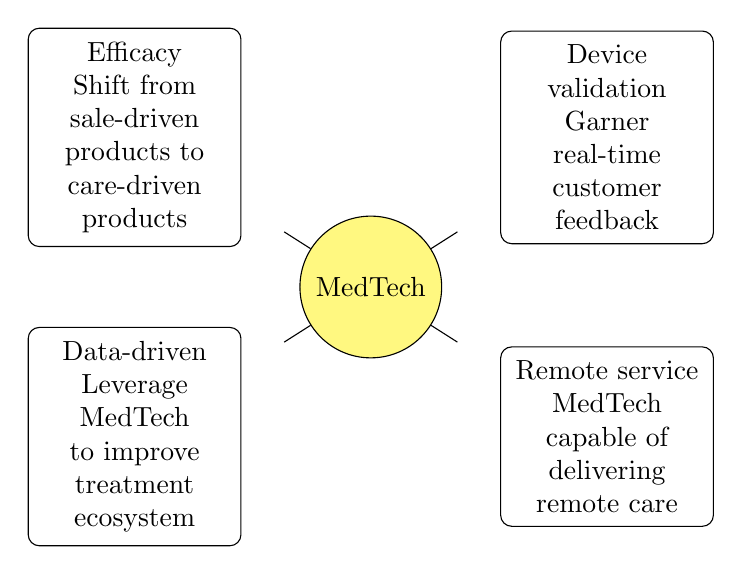
\begin{tikzpicture}
\node[draw, circle, minimum size=1.8cm, align=center, fill=yellow!50] (m) at (0,0) {MedTech};

\node[draw, rounded corners, align=center, text width=2.35cm, inner sep=5pt] (e) at (-3.0,1.9)
{Efficacy\\Shift from sale-driven\\products to care-driven\\products};

\node[draw, rounded corners, align=center, text width=2.35cm, inner sep=5pt] (d) at (-3.0,-1.9)
{Data-driven\\Leverage MedTech\\to improve treatment\\ecosystem};

\node[draw, rounded corners, align=center, text width=2.35cm, inner sep=5pt] (v) at (3.0,1.9)
{Device validation\\Garner real-time\\customer feedback};

\node[draw, rounded corners, align=center, text width=2.35cm, inner sep=5pt] (r) at (3.0,-1.9)
{Remote service\\MedTech capable of\\delivering remote care};

\draw (m) -- (-1.1,0.7);
\draw (m) -- (-1.1,-0.7);
\draw (m) -- (1.1,0.7);
\draw (m) -- (1.1,-0.7);
\end{tikzpicture}
\caption{Pocket-safe redraw of the MedTech framework visible in the lecture slide.}
\end{figure}

\subsection{Question \& Answer}

\paragraph{Question.} Why is ``safe and effective'' still not enough?

\paragraph{Answer.} Because the commercial system is not the same as the technical system. In med tech one must ask who adopts first, which clinicians are influential, how quickly the relevant specialty changes behavior, who pays, whether the product can be prescribed, and whether direct-to-consumer demand matters at all. A direct-to-consumer advertisement may create awareness, but if the physician does not prescribe, the product does not move. The model must therefore include not only efficacy and safety, but adoption, validation, reimbursement, and service structure.

The lecture then widens again, but now the late examples land differently because the general principle is clear. Switching costs become a useful asymmetry:
\begin{equation}
\text{low switching cost for buyer}
\Rightarrow
\text{high churn risk for seller}.
\end{equation}
This is illustrated through mobile carriers and fitness memberships. Buyers prefer easy exit; sellers fear it. Mint Mobile then appears as a segmentation move layered on top of T-Mobile's infrastructure: a cheaper, lower-bandwidth, more flexible offer reaches a part of the market that the main branded offer does not.

The same logic reappears in brand ladders. Toyota reaches one class of customer; Lexus reaches another. Ralph Lauren holds multiple levels of aspiration under one umbrella. The lecture's live exchange on automotive brand genealogy is somewhat muddled, but the central point is firm: a company with a successful model may still need a second label or second offer to reach a segment that the original identity cannot capture.

The remaining examples continue the same motif in quicker strokes. Uber and Airbnb show platform coordination without direct ownership of the core asset. Rent the Runway shows a personalized subscription logic rather than a simple sharing logic. Amazon replenishment shows how smart sensing and subscription remove the friction of remembering to buy. Travel planning shows how AI can move from search assistance to itinerary construction. The Norwegian data-center example sharpens the difference between a business and a business model: a data center is an asset, but a data center in a cold region, financed in a certain way, powered in a certain way, and tied to a particular compute contract is a business model. Otter then appears as an application-side example in which transcription becomes summary and summary becomes action.

The closing advice therefore has real force behind it. Do not overcomplicate the model. Understand the market dynamics. Be flexible. The companies that survive are the ones that alter themselves before the world forces the alteration upon them.

\section{Summary}

The lecture begins with customer discovery and ends with adaptability. In between, it teaches three durable lessons. First, a business model is the coupled structure by which value is created, delivered, and captured. Second, the route to market is as consequential as the product itself; the MolecularWare case makes this plain. Third, successful firms modify their models before the old ones fail outright. Netflix does this across format and content. Google does it by turning service into predictive data. MedTech reveals the sharpest form of the problem: technical success does not guarantee adoption. The final note is therefore practical rather than grand. We should look at every company and ask not only what it makes, but how it reaches the buyer, how it gets paid, and how it will change when the present arrangement is no longer enough.